% !TEX root = main.tex

\section{搜索}
搜索主要包括无信息(uninformed)搜索和有信息搜索。
\begin{itemize}
	\item 状态空间(state space)
	\begin{itemize}
		\item 传统搜索:状态空间可见、动作确定性
		\item 非传统搜索:局部搜索、模拟退火、爬坡
	\end{itemize}
	\item 动作(action):不同状态之间的转换
	\item 初始状态(initial state)
	\item 目标/期望(goal)
\end{itemize}
% 对抗搜索(adversarial):博弈树(minimax)、$\alpha-\beta$剪枝

树搜索,边界集(frontier)是未探索的状态集合
\begin{algorithm}[H]
\caption{Tree Search}
\begin{algorithmic}[1]
\Procedure{TreeSearch}{(Frontier, Successors, Goal?)}
\If{Frontier is empty}
\State \Return failure
\EndIf
\State Curr $=$ select state from Frontier
\If{Goal?(Curr)}
\State \Return Curr
\EndIf
\State $\text{Frontier'} = (\text{Frontier} - \{\text{Curr}\}) \cup \text{Successors(Curr)}$
\State \Return TreeSearch(Frontier',Successors,Goal?)
\EndProcedure
\end{algorithmic}
\end{algorithm}

搜索需要关注的几个特性:
\begin{itemize}
	\item 完备性:若解存在,搜索是否总能找到解
	\item 最优性:是否总能找到最小代价的解
	\item 时间复杂性:最大需要被\textbf{生成或展开}\footnote{而不是探索的结点数目}的结点数
	\item 空间复杂性:最大需要被存储在内存中的结点数
\end{itemize}

\subsection{无信息搜索}
\subsubsection{宽度优先搜索(BFS)}
将后继加入边界集的后面,$b$为最大状态后继数目/分支因子(branching factor),$d$为最短距离解的行动数(注意是\textbf{边数},而不是层数!)
\begin{itemize}
	\item 完备性与最优性:所有短路总在长路前被探索,某一长度只有有限多条路径,最终可以检测所有长度为$d$的路径,从而找到最优解
	\item 时间复杂度:$1+b+b^2+\cdots+b^d+(b^d-1)b=O(b^{d+1})$,最差情况在最后一层的最后一个节点才探索到最优解,从而前面$b$个节点都要展开第$d+1$层
	\item 空间复杂度:$b(b^d-1)=O(b^{d+1})$,需要将边界集都存储下来
\end{itemize}

\subsubsection{深度优先搜索(DFS)}
将后继加入边界集的前面,即总是展开边界集中最深的节点
\begin{itemize}
	\item 完备性
	\begin{itemize}
		\item 无限状态空间:不能保证
		\item 有限状态空间无限路径:不能保证
		\item 有限状态空间+路径/重复状态剪枝:可以保证
	\end{itemize}
	\item 最优性:因完备性不能保证,故最优性也不能保证
	\item 时间复杂性:$O(b^m)$,其中$m$为状态空间的最长路的长度(若$m>>d$,则非常糟糕;但如果有大量解路径,则会快于BFS)
	\item 空间复杂性:$O(bm)$,\textbf{线性空间复杂性}是DFS最大的优点。边界集只包含当前路径的最深节点以及回溯节点(backtrack points为当前路径上节点的未探索的兄弟sibling)
\end{itemize}

\subsubsection{一致代价(Uniform-cost)}
一致代价搜索(Uniform cost search, UCS)\footnote{至于为什么叫Uniform,可以看\url{https://math.stackexchange.com/questions/112734/in-what-sense-is-uniform-cost-search-uniform}和\url{https://cs.stackexchange.com/questions/6072/why-is-uniform-cost-search-called-uniform-cost-search},比较合理的解释是到达同一结点的cost都被认为是相同的(寻找最优解时)。一致的算法总是选择边界集中第一个元素。}的边界集以路径开销升序排序,总是先展开最低开销的路径。
如果每一个动作都是一样的代价,则一致代价等价于BFS。
\begin{itemize}
	\item 完备性与最优性:假设所有转移都有代价$\geq\eps>0$,所有更低代价的路径都在高代价路径之前被展开,只有有限多的路径开销小于最优解的开销,故最终一定会到达最优解
	\item 时间复杂性:$O(b^{C^\star/\eps+1})$,对应着BFS中$d=C^\star/\eps$,其中$C^\star$为最优解的开销,最坏情况就是每一层开销都很小为$\eps$
	\item 空间复杂性:$O(b^{C^\star/\eps+1})$
\end{itemize}

\subsubsection{深度受限搜索(Depth-limited)}
执行只在最大深度执行DFS,因此无穷路径长不会存在问题
\begin{itemize}
	\item 完备性与最优性:不能保证,若解的深度大于$L$
	\item 时间复杂度:$O(b^L)$
	\item 空间复杂度:$O(bL)$
\end{itemize}

\subsubsection{迭代加深搜索(Iterative Deepening)}
迭代加深搜索(Iterative Deepening Searching, IDS)逐渐增加最大深度$L$,对每一个$L$做深度受限搜索
\begin{itemize}
	\item 完备性:可以保证
	\item 最优性:如果开销一致\footnote{若开销不一致,则可以采用代价界(cost bound)来代替:仅仅展开那些路径开销小于代价界的路径,同时要记录每一层深搜的最小代价。这种方式的搜索开销会非常大,有多少种不同路径开销就需要多少次迭代循环。},则可以保证
	\item 时间复杂性:$(d+1)b^0+db+(d-1)b^2+\cdots+b^d=O(b^d)$,第$0$层搜了$(d+1)$次,可以看到时间复杂度是\textbf{比BFS优}的
	\item 空间复杂性:$O(bd)$,同DFS
\end{itemize}

\subsubsection{双向搜索(Bidirectional)}
从源结点和汇结点同时采用BFS,直到两个方向的搜索汇聚到中间。
\begin{itemize}
	\item 完备性:由BFS保证
	\item 最优性:若一致代价则可保证
	\item 时间复杂性:$O(b^{d/2})$
	\item 空间复杂性:$O(b^{d/2})$
\end{itemize}

\subsubsection{环路/路径检测}
\begin{itemize}
	\item 环路(cycle)检测:检测当前状态是否与已探索的状态重复(BFS)
	\item 路径(path)检测:只检测当前状态是否与该路径上的状态重复(DFS)
\end{itemize}
注意不能将环路检测运用在BFS上,因为开销太大。

环路检测运用到UCS上依然\textbf{可以保证最优性}\footnote{注意这在启发式搜索中不一定成立}。
因为UCS第一次探索到某一状态的时候已经发现最小代价路径,因而再次探索该状态不会发现路径比原有的更小。

\subsubsection{总结}
\begin{center}
\begin{tabular}{ccccccc}\hline
& BFS & UCS & DFS & Depth-limited & IDS & Bidirectional\\\hline
完备性 & \cmark & \cmark & \xmark & \xmark & \cmark & \cmark\\
时间复杂度 & $O(b^d)$ & $O(b^{\lfloor C^\star/\eps\rfloor+1})$ & $O(b^m)$ & $O(b^l)$ & $O(b^d)$ & $O(b^{d/2})$\\
空间复杂度 & $O(b^d)$ & $O(b^{\lfloor C^\star/\eps\rfloor+1})$ & $O(bm)$ & $O(bl)$ & $O(bd)$ & $O(b^{d/2})$\\ 
最优性 & \cmark & \cmark & \xmark & \xmark & \cmark & \cmark\\\hline
\end{tabular}
\end{center}

\begin{example}
$N$个传教士和$N$个食人族要过河,他们都在河的左岸。
现在只有一条船能够运载$K$个人,要把他们都运往右岸。
要满足无论何时何地,传教士的数目都得大于等于食人族的数目,或者传教士数目为0。
\end{example}
\begin{analysis}
考虑对问题形式化为搜索问题
\begin{itemize}
	\item 状态$(M,C,B)$,其中$M$为左岸传教士数目,$C$为左岸食人族数目,$B=1$指船在左岸
	\item 动作$(m,c)$指运$m$个传教士和$c$个食人族到对岸
	\item 先决条件:传教士数目和食人族数目满足限制
	\item 效果:$(M,C,1)\stackrel{(m,c)}{\implies}(M-m,C-c,0)$\\
	$(M,C,0)\stackrel{(m,c)}{\implies}(M+m,C+c,1)$
\end{itemize}
\end{analysis}

\subsection{有信息搜索}
在无信息搜索中,我们从不估计边界集中最有期望(promising)获得最优解的结点,而是无区别地选择当前边界集中第一个结点。
然而事实上,针对不同问题我们是有对结点的先验知识(apriori knowledge)的,即从当前结点到目标结点的开销有多大。
而这就是有信息搜索(informed),或者称为启发式搜索(heuristics)。

关键在于领域特定启发式函数$h(n)$的设计,它估计了从结点$n$到目标结点的开销(cost)。
注意满足目标状态的结点$h(n)=0$。

\subsubsection{贪心最优搜索(Greedy Best-First Search)}
直接使用$h(n)$对边界集进行排序,但这会导致贪心地选择\textbf{看上去}离目标结点开销最小的路径。

如果存在环路,贪心最优搜索是不完备的,会陷入死循环。

\subsubsection{A$^\star$搜索}
综合考虑当前已走的开销和未来估计的开销。
定义一个估值函数
\[f(n)=g(n)+h(n)\]
其中$g(n)$为路径到节点$n$的代价,$h(n)$为从$n$到目标节点的代价,采用$f(n)$对边界集内的节点进行排序。

$f(n)$需要满足下列两个性质。
\begin{definition}[可采纳的(admissibility)]
假设所有代价$c(n1\to n2)\geq\eps>0$,令$h^\star(n)$为从$n$到目标节点$\infty$的最优解\footnote{如果没有路径则$h^\star(n)=\infty$},若
\[\forall n:\;h(n)\leq h^\star(n)\]
则称$h(n)$是可采纳的。
即一个可采纳的启发式函数总是\textbf{低估}了当前结点到目标结点的真实开销(这样才能保证最优解不被排除)。
\end{definition}
\begin{definition}[一致性(consistency)/单调性(monotonicity)]
若对于所有的结点$n_1$和$n_2$,$h(n)$满足(三角不等式)
\[h(n_1)\leq c(n_1\to n_2)_h(n_2)\]
则称$h(n)$是单调的。
\end{definition}

\begin{theorem}
一致性蕴含可采纳性
\end{theorem}
\begin{analysis}
分类讨论
\begin{itemize}
	\item 当结点$n$没有到目标结点的路径,则$h(n)\leq h^\star(n)=\infty$恒成立
	\item 令$n=n_1\to n_2\to\cdots\to n_k$为从结点$n$到目标结点的最优路径,则可以用数学归纳法证明$\forall i:\;h(n_i)\leq h^\star(n_i)$,如下从后往前推
	\[h(n_{i})\leq c(n_i\to n_{i+1})+h(n_{i+1})\leq c(n_i\to n_{i+1}) + h^\star(n_{i+1})=h^(n_i)\]
\end{itemize}
\end{analysis}

\begin{theorem}
可采纳性蕴含最优性
\end{theorem}
\begin{analysis}
假设最优解有开销$C^\star$,则任何最优解一定会在开销大于$C^\star$的路径之前被展开。
因此在最优解展开之前的路径一定有开销$\leq C^\star$,最终我们一定会检测到最优解,而且次优解不会在最优解之前被检测。
\end{analysis}

做环检测可能导致找不到最优解

但如果满足单调性,有以下几个性质
\begin{proposition}
路径上的$f$一定是非递减的
\end{proposition}
\begin{analysis}
\[\begin{aligned}
f(n)&=g(n)+h(n)\\
&\leq g(n)+c(n\to n')+h(n')\\
&= g(n')+h(n')\\
&= f(n')
\end{aligned}\]
\end{analysis}

\begin{proposition}
如果$n_2$在$n_1$之后被扩展,则$f(n_1)\leq f(n_2)$
\end{proposition}
\begin{analysis}
$n_2$在边界上
$n_1$
\end{analysis}
\begin{proposition}
当$n$在任何小于$f$值得路径之前被展开
\end{proposition}
\begin{analysis}
\end{analysis}
\begin{proposition}
$A^\star$算法第一次展开某个状态时,它已经找到了到达那个状态的最小开销路径。
\end{proposition}
\begin{analysis}
\end{analysis}

若满足单调性,则进行环检测不会破坏最优性

\subsubsection{迭代加深$A^\star$(IDA)算法}
$A^\star$算法有和BFS或UCS同样的空间复杂性问题,而迭代加深$A^\star$算法同样解决空间复杂度的问题

\subsubsection{构造启发式函数}
常常需要考虑一个更加简单的问题,然后让$h(n)$为到达一个简单问题解的开销

\begin{example}
现有积木若干,积木可以放在桌子上,也可以放在另一块积木上面。
有两种操作:
\begin{enumerate}
	\item \verb'move(x,y)':把积木x放到积木y上面,前提是积木x和积木y上面都没有其他积木
	\item \verb'moveToTable(x)':把积木x放到桌子上,前提是积木x上面无其他积木,且积木x不在桌子上
\end{enumerate}
设计一个可采纳的启发式函数$h(n)$
\end{example}
\begin{analysis}
$h(n)=h_1(n)+h_2(n)$
\end{analysis}

\subsection{博弈树搜索}
博弈的一些前提
\begin{itemize}
	\item 两个博弈玩家
	\item 离散值:游戏和决策都可以映射到离散空间
	\item 有限的:只有有限的状态和可能的决策
	\item 零和博弈:完全竞争,即如果一个玩家胜利,则另外一个失去同样数量的收益
	\item 确定性的:没有牵涉到概率性事件,如色子、抛硬币等
	\item 完美信息博弈:状态的所有方面都可以被完全观察,即没有隐藏的卡牌
\end{itemize}

剪刀石头布是简单的一次性(one-shot)博弈
\begin{itemize}
	\item 一次移动
	\item 在博弈论中称为策略或范式博弈(strategic/normal form)
\end{itemize}

但很多游戏是牵涉到多步操作的
\begin{itemize}
	\item 轮回(turn-taking)游戏,如棋类
	\item 在博弈论中称为扩展形式博弈(extensive form)
\end{itemize}

两个玩家$A$(最大化己方收益)和$B$(最小化对方收益)
\begin{itemize}
	\item 状态集合$\mathcal{S}$
	\item 初始状态$I\in\mathcal{S}$
	\item 终止位置$T\subset\mathcal{S}$
	\item 后继:下一可能状态的集合
	\item 效益(utility)/收益(payoff)函数$V:T\mapsto\rr$,表明终止状态对$A$玩家有多好,对$B$玩家有多坏(都站在$A$角度给出)
\end{itemize}

minimax算法:自己选max,对方选min
\begin{itemize}
	\item 构建整棵博弈树,然后将终止/叶子结点标上收益
	\item 回溯整棵树,然后将每个结点都标记上收益
\[U(n)=
\begin{cases}
\min\{U(c):\;c \text{ is a child of } n\} & n \text{ is a Min node}\\
\max\{U(c):\;c \text{ is a child of } n\} & n \text{ is a Max node}
\end{cases}\]
\end{itemize}
\begin{figure}[H]
\centering
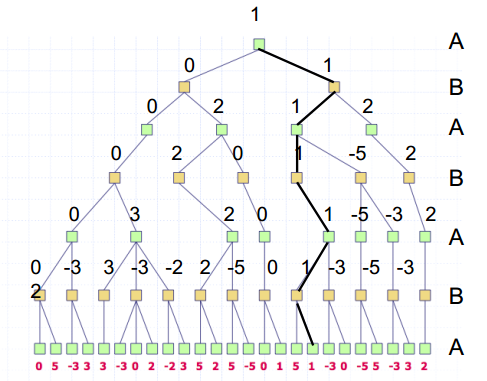
\includegraphics[width=0.6\linewidth]{fig/game-tree.png}
\end{figure}

用DFS可以遍历整棵树,同时保持线性的空间复杂度,每次回溯时更新结点为min/max即可

$\alpha$-$\beta$剪枝
\begin{itemize}
	\item 只要当前Max结点的值$\geq$祖先某一Min结点的值,就可以在该Max结点上做$\alpha$剪枝
	\item 只要当前Min结点的值$\leq$祖先某一Max结点的值,就可以在该Min结点上做$\alpha$剪枝
\end{itemize}
\begin{algorithm}
\caption{Alpha-Beta Pruning}
\begin{algorithmic}[1]
\Procedure{AlphaBeta}{n,Player,alpha,beta}
\If{n is TERMINAL}
\State \Return V(n)\Comment{Return terminal states utility}
\EndIf
\State ChildList = n.Successors(Player)
\If{Player == MAX}
\For{c in ChildList}
\State alpha = max(alpha, AlphaBeta(c,MIN,alpha,beta))
\If{beta <= alpha}
\State break
\EndIf
\EndFor
\State \Return alpha
\Else\Comment{Player == MIN}
\For{c in ChildList}
\State beta = min(beta, AlphaBeta(c,MAX,alpha,beta))
\If{beta <= alpha}
\State break
\EndIf
\EndFor
\State \Return beta
\EndIf
\EndProcedure\Comment{Initial call: AlphaBeta(START-NODE,Player,$-\infty$,$+\infty$)}
\end{algorithmic}
\end{algorithm}
可以证明,如果原始情况需要访问$O(b^D)$个结点,则经过$\alpha$-$\beta$剪枝后只需访问$O(b^{D/2})$个结点。

但在现实生活的游戏中,即使采用了$\alpha$-$\beta$剪枝,博弈树也太过庞大。
如棋类的分支因子大致是35,深度为10的树已经到$2.7\times 10^{14}$个结点。
因此不能将整棵博弈树展开,需要采用一些启发式方式进行估计。

评价函数(evaluation)的一些需求:
\begin{itemize}
	\item 对于终止状态,评价函数的序应与真实的收益函数相同
	\item 对于非终止状态,评价函数则应该与真实的胜率相关联
	\item 计算时间不能花太长
	\item 通常取多个特征,然后进行加权求和(先验知识)
\end{itemize}

在线(online)/实时(real-time)搜索
\begin{itemize}
	\item 没有办法展开全部的边界集,因此限制展开的大小(在没找到去目标的真实路径就做出决定/直接选一条路就开始走)
	\item 在这种情况下,评价函数不仅仅引导搜索,更是提交真实的动作
	\item 虽然找不到最优解,但是求解时间大大缩减
\end{itemize}